\section{The optimal universal real-order Euler bound}
\label{sec:euler}

Let
\begin{equation}\label{eul:eq:definitions}
 A_k=\frac{H_{2k}^{(b)}}{(2k+1)^a},\qquad
 d_j=\sum_{k=0}^{j}(-1)^k\binom{j}{k}A_k,\qquad
 E_N=\sum_{j=0}^{N-1}\frac{d_j}{2^{j+1}},\qquad
 g_{a,b}=\Im F_{a,b}(i).
\end{equation}
Thus $A_0=d_0=E_1=0$. The Euler transformation itself is classical
\cite{DLMFeuler}. The issue addressed here is a parameter-uniform
bound with the correct analytic interpretation, including parameter
values for which the untransformed alternating series diverges.

\begin{theorem}[Sharp universal Euler constant]\label{eul:thm:main}
For all $a,b>0$ the Euler series is absolutely convergent and $E_N$
decreases strictly to $g_{a,b}$ for $N\ge1$. Moreover,
\begin{equation}\label{eul:eq:universal-nine-eighths}
 0<E_N-g_{a,b}<\frac98\,2^{-N}\qquad(N\ge2).
\end{equation}
Define
\begin{equation}\label{eul:eq:Cstar}
 C_* =\max_{b>0}C(b),\qquad
 C(b)=\beta(b)+2^{-b}\eta(b).
\end{equation}
Then
\begin{equation}\label{eul:eq:sharp-universal}
 0<E_N-g_{a,b}<C_*2^{-N}\qquad(a,b>0,\ N\ge1),
\end{equation}
and no smaller constant works simultaneously for all these parameters.
The maximum in \eqref{eul:eq:Cstar} is attained at exactly one
$b=b_*\in(1,2)$, as in the Gaussian axis theorem of the baseline.
On the closure $a\ge0,b>0$, equality in the corresponding non-strict
bound occurs only at $a=0$, $b=b_*$, $N=1$.
\end{theorem}

Numerically,
\[
 b_*\approx1.30221658710124120959,\qquad
 C_*\approx1.13656110333950956095.
\]
These decimals are diagnostics, not the definition of the constant.
The rigorous result is the exact maximum in \eqref{eul:eq:Cstar},
its unique maximizer, and the rational bound \eqref{eul:eq:universal-nine-eighths}.
The latter is particularly convenient for certification: practical
evaluations use $N\ge2$, so they need no evaluation of $C_*$.

\begin{figure}[htbp]
\centering
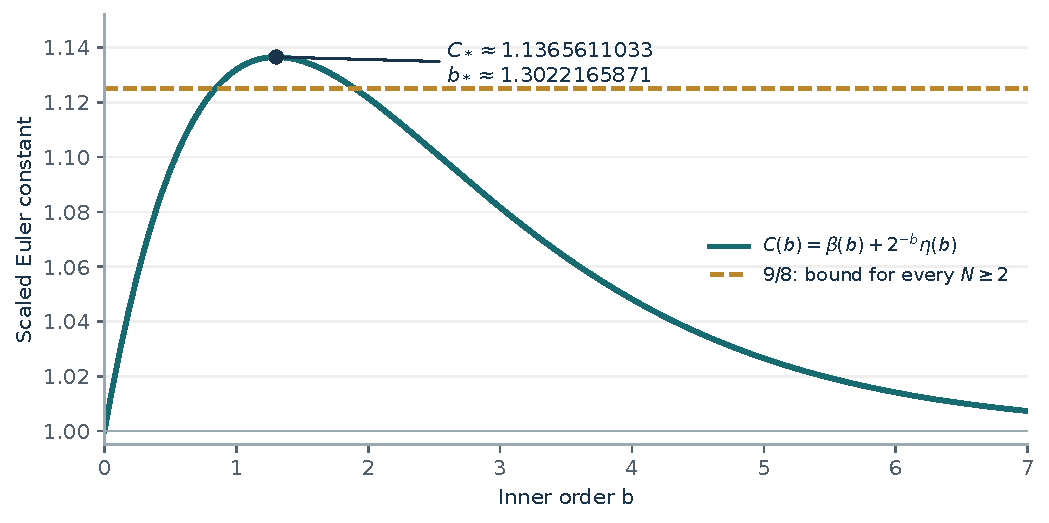
\includegraphics[width=.88\linewidth]{figures/euler_axis.pdf}
\caption{The inherited axis function and the new strict separator for
every later Euler step. The curve is a numerical illustration; the
maximum is defined exactly by \eqref{eul:eq:Cstar}, and the separation
from $9/8$ has the rational witness \eqref{eul:eq:C-lower}.}
\label{eul:fig:axis}
\end{figure}

\subsection{A probability representation with no threshold}

For $s>0$ let $\mu_s$ be the probability measure on $(0,1)$ with density
\begin{equation}\label{eul:eq:mu}
 d\mu_s(x)=\frac{(-\log x)^{s-1}}{\Gamma(s)}\,dx.
\end{equation}
Equivalently, $X_s=e^{-T_s}$ where $T_s$ is gamma distributed with
shape $s$ and rate one. The elementary gamma integral gives
\[
 \int_0^1x^{n-1}\,d\mu_s(x)=n^{-s}\qquad(n>0).
\]
At $s=0$, when needed, set $\mu_0=\delta_1$.

\begin{lemma}[Positive double integral]\label{eul:lem:positive}
For independent $X\sim\mu_a$ and $Y\sim\mu_b$,
\begin{align}
 A_k&=\E\!\left[X^{2k}\frac{1-Y^{2k}}{1-Y}\right],\label{eul:eq:moment}\\
 F_{a,b}(z)&=z^2\E\!\left[
       \frac{X}{(1-zX)(1-zXY)}\right]
       \qquad(z\in\C\setminus[1,\infty)).\label{eul:eq:F-integral}
\end{align}
In particular,
\begin{equation}\label{eul:eq:gaussian-integral}
 -g_{a,b}=\E\!\left[
 \frac{X^2(1+Y)}{(1+X^2)(1+X^2Y^2)}\right]>0.
\end{equation}
These formulas also hold for $a=0,b>0$.
\end{lemma}
\begin{proof}
Expand $(1-Y^m)/(1-Y)=\sum_{r=0}^{m-1}Y^r$ and apply the gamma
moment formula. This proves \eqref{eul:eq:moment}. For $|z|<1$, absolute
convergence permits summation of the two geometric series in
\[
 \E\!\left[\frac{z}{1-Y}
     \left\{\frac1{1-zX}-\frac1{1-zXY}\right\}\right].
\]
Their difference is exactly the integrand in \eqref{eul:eq:F-integral}.
On a compact subset of the slit plane, both denominators stay uniformly
away from zero for $X,Y\in[0,1]$. The probability integral is therefore
holomorphic there and supplies the asserted principal continuation.
At $z=i$, rationalization gives \eqref{eul:eq:gaussian-integral}.
No signed-moment existence theorem is required.
\end{proof}

\begin{lemma}[Exact positive Euler tail]\label{eul:lem:tail}
Set
\begin{equation}\label{eul:eq:W-K}
 W_N(x)=\frac{(1-x^2)^N}{1+x^2},\qquad
 \mathcal K_N(x,y)=\frac{W_N(xy)-W_N(x)}{1-y}.
\end{equation}
Then, for every $N\ge1$,
\begin{equation}\label{eul:eq:tail}
 2^N(E_N-g_{a,b})=\E[\mathcal K_N(X,Y)].
\end{equation}
The integrand is strictly positive for $0<x,y<1$.
\end{lemma}
\begin{proof}
Apply the binomial theorem to the finite expression in
\eqref{eul:eq:moment}:
\begin{equation}\label{eul:eq:negative-increments}
 d_j=\E\!\left[
 \frac{(1-X^2)^j-(1-X^2Y^2)^j}{1-Y}\right]<0\qquad(j\ge1).
\end{equation}
For $u,v\in[0,1]$ the inequality $|u^j-v^j|\le j|u-v|$ gives
$|d_j|\le2j$. Thus the Euler series converges absolutely, uniformly
under the probability integral. Summing it gives
\[
 \sum_{j\ge0}2^{-j-1}d_j
 =\E\!\left[\frac{(1+X^2)^{-1}-(1+X^2Y^2)^{-1}}{1-Y}\right]
 =g_{a,b}.
\]
Summing only the terms $j\ge N$ yields \eqref{eul:eq:tail}. Since
$W_N$ is strictly decreasing on $(0,1)$, the sign is strict. The same
argument works at $a=0$, because then $X=1$ while $0<Y<1$.
\end{proof}

The identity \eqref{eul:eq:tail} separates the uniform problem into
an elementary kernel inequality and a probability average. Its first
case is
\begin{equation}\label{eul:eq:K1}
 \mathcal K_1(x,y)=
 \frac{2x^2(1+y)}{(1+x^2)(1+x^2y^2)}.
\end{equation}
The behavior of the later kernels is sufficiently different that
their bounds cannot be inferred solely from the size of $g_{a,b}$.

\subsection{Three polynomial inequalities control every later tail}

\begin{lemma}[Uniform kernel gap]\label{eul:lem:kernel-gap}
For every integer $N\ge2$, $0\le x\le1$, and $0\le y<1$,
\begin{equation}\label{eul:eq:kernel-gap}
 0\le\mathcal K_N(x,y)<\frac98.
\end{equation}
The same upper bound holds at $y=1$ by the continuous limiting value.
\end{lemma}

We give the reduction and all finite premises of the proof. Put $u=x^2$.
For $N=2,3$, define the polynomial
\begin{align}\label{eul:eq:PN}
 P_N(u,y)={}&9(1+u)(1+uy^2)\\
 &-8\frac{(1-uy^2)^N(1+u)-(1-u)^N(1+uy^2)}{1-y}.\notag
\end{align}
The numerator vanishes at $y=1$, so the quotient is a polynomial.
Direct division gives
\begin{align}\label{eul:eq:P2}
 P_2={}&9+u(9y^2-24y-15)\notag\\
 &+u^2(8y^3+17y^2+8y+8)+8u^3(y^3+y^2),
\end{align}
and
\begin{align}\label{eul:eq:P3}
 P_3={}&9+u(9y^2-32y-23)
       +u^2(24y^3+33y^2+24y+24)\notag\\
 &+u^3(-8y^5-8y^4+16y^3+16y^2-8y-8)\notag\\
 &-8u^4(y^5+y^4+y^3+y^2).
\end{align}
Exact positive Bernstein expansions on dyadic boxes prove
$P_2>0$ and $P_3>0$ on the closed unit square. Since
\[
 \frac98-\mathcal K_N(x,y)
 =\frac{P_N(x^2,y)}{8(1+x^2)(1+x^2y^2)},
\]
these prove the first two cases of the kernel lemma.

For $N\ge4$, write
$w_N(t)=(1-t)^N/(1+t)$ for $0\le t\le1$. Every derivative has the
alternating sign appropriate to its order: Leibniz's formula is a
sum of products of two factors with that property. Also
$w_N^{(j)}(1)=0$ for $j=0,1,2,3$. Taylor's formula with integral
remainder consequently gives
\begin{equation}\label{eul:eq:mixture}
 w_N(t)=\int_{(0,1]}(1-t/s)_+^4\,d\sigma_N(s),
\end{equation}
where
\begin{equation}\label{eul:eq:mixture-measure}
 d\sigma_N(s)=\frac{-s^4w_N^{(5)}(s)}{24}\,ds
             +\frac{w_N^{(4)}(1)}{24}\,\delta_1(ds).
\end{equation}
It is a positive measure, and setting $t=0$ shows that its mass is
$w_N(0)=1$. The atom has mass $1/2$ for $N=4$ and is absent for
$N>4$. This elementary truncated-power representation is a special
case of the classical multiply monotone framework
\cite{Williamson,McNeilNeslehova}; here Taylor's formula proves exactly
the representation used, including its endpoint atom.

For fixed $0<y<1$, the largest value over $r\ge0$ of
\[
 \frac{(1-r^2y^2)_+^4-(1-r^2)_+^4}{1-y}
\]
occurs at
\[
 r^2=\frac{1-y^{2/3}}{1-y^{8/3}}<1.
\]
Indeed, in $0<r<1$ differentiation in $r^2$ gives this unique critical
point, with derivative positive before it and negative afterwards.
For $r\ge1$ the expression is decreasing until it becomes zero.
Its maximum is therefore
\begin{equation}\label{eul:eq:M4}
 M_4(y)=\frac{(1-y)^3(1+y)^4}{(1-y^{8/3})^3}.
\end{equation}
The limiting values at $y=0,1$ are also finite. Set $y=v^3$ and
define
\begin{equation}\label{eul:eq:Q4}
 Q_4(v)=\frac{9(1-v^8)^3-8(1-v^3)^3(1+v^3)^4}{(1-v)^3}.
\end{equation}
The expression is a polynomial of degree 21. Two exact Bernstein
expansions, on $[0,1/2]$ and $[1/2,1]$, have strictly positive
coefficients. Hence $M_4(y)<9/8$ for $0\le y<1$, and the limiting
case also satisfies the strict bound. Substitute \eqref{eul:eq:mixture}
into \eqref{eul:eq:W-K}, with $r=x/\sqrt{s}$. This ratio may exceed
one, which is why the preceding maximization included all $r\ge0$.
A probability average of quantities bounded by $M_4(y)$ proves
\eqref{eul:eq:kernel-gap} for all $N\ge4$.

\subsection{The finite positivity certificates}

For clarity, the proof certificate does not use a numerical polynomial
optimizer. If $p(t)=\sum_{j=0}^{d}a_jt^j$, its degree-$d$ Bernstein
coefficients on $[0,1]$ are
\begin{equation}\label{eul:eq:bernstein}
 b_k=\sum_{j=0}^{k}a_j\frac{\binom{k}{j}}{\binom{d}{j}},\qquad
 p(t)=\sum_{k=0}^{d}b_k\binom{d}{k}t^k(1-t)^{d-k}.
\end{equation}
The basis functions are nonnegative and sum to one. For a box in
several variables, first make an affine substitution to the unit box
and then apply the formula in each variable. Positivity of every
coefficient proves strict positivity on the whole closed box.

The standard-library verifier \src{code/certify_euler_bound.py}
constructs the three polynomials directly from
\eqref{eul:eq:PN} and \eqref{eul:eq:Q4}, checking each exact polynomial
division. It recursively bisects a box only when its current
Bernstein coefficients do not already prove positivity. The resulting
finite partition and its exact rational lower coefficients are written
to \src{data/euler_polynomial_certificate.json}.

\begin{center}
\begin{tabular}{@{}lrrl@{}}
\toprule
Polynomial & Boxes & Positive coefficients & Smallest coefficient\\
\midrule
$P_2$ & 13 & 208 & $3/64$\\
$P_3$ & 7 & 210 & $11337/40960$\\
$Q_4$ & 2 & 44 & $1$\\
\bottomrule
\end{tabular}
\end{center}

Thus the proof uses 462 positive rational coefficients in total.
An independent SymPy verifier reconstructs the expressions without
importing the producer's polynomial operations, checks all coefficients,
checks that box interiors are disjoint, and checks that their total
volume is one. The producer's recursive bisection already ensures
coverage; the independent checks also make the stored partition
directly reviewable.

\subsection{Why the first step determines the exact optimum}

For fixed $y\in(0,1)$, \eqref{eul:eq:K1} is strictly increasing in
$x\in(0,1)$, because its derivative has the positive factor
$1-x^4y^2$. Consequently
\begin{equation}\label{eul:eq:axis-domination}
 -2g_{a,b}=\E[\mathcal K_1(X,Y)]
 <\E\!\left[\frac{1+Y}{1+Y^2}\right]=C(b)
 \qquad(a>0).
\end{equation}
The equality on the right follows either from the axis formula
$F_{0,b}(z)=z\Li_b(z)/(1-z)$ or by the convergent residue-class
definitions of $\beta$ and $\eta$. As $a\downarrow0$, $X\to1$
in probability, so bounded convergence gives equality in the limit.

The following prerequisite was already proved in the baseline. We
include its principal argument to make the use of the maximum
self-contained.

\begin{proposition}[The inherited axis maximum]\label{eul:prop:axis}
The function $C$ in \eqref{eul:eq:Cstar} has exactly one stationary
point on $(0,\infty)$. It is a nondegenerate global maximum. Moreover,
$C(b)>1$ for finite $b>0$, and $C(b)\to1$ at both ends of the interval.
\end{proposition}
\begin{proof}
Let $\varphi(T)=(1+e^{-T})/(1+e^{-2T})$. Then
$C(b)=\E[\varphi(T_b)]$. The function $\varphi$ increases and then
decreases, its unique maximum being at $T=\log(1+\sqrt2)$.
It is larger than one and at most $(1+\sqrt2)/2$ for finite $T>0$.
Gamma concentration at zero as $b\downarrow0$, and at infinity as
$b\to\infty$, gives the endpoint limits and existence of a maximum.

For $1<\lambda<\max\varphi$, the function
$f(T)=\varphi(T)-\lambda$ has exactly two sign changes $T_1<T_2$,
with signs negative, positive, negative. It is impossible that
$C(b_j)=\lambda$ at three distinct $b_1<b_2<b_3$. To see this, put
$v=T^{b_2-b_1}$ and $p=(b_3-b_1)/(b_2-b_1)>1$.
Subtract from $v^p$ the secant line through its values at $T_1,T_2$,
and multiply by $-T^{b_1-1}$. Strict convexity produces a linear
combination of the three powers $T^{b_j-1}$ with the same strict
sign pattern as $f$. Its integral against $f(T)e^{-T}$ is positive,
contradicting the three vanishing Mellin integrals.

At a stationary point $b_0$, put $\lambda=C(b_0)$. If $C''(b_0)=0$
as well, the Mellin integral of $f$ and its first two derivatives in
$b$ vanish. Their linear combination with kernel
\[
 -T^{b_0-1}(\log T-\log T_1)(\log T-\log T_2)
\]
again gives a strictly positive integral, a contradiction. Every
stationary point is therefore nondegenerate. A local minimum would
give three intersections with its horizontal level, since the two
endpoint limits are lower; hence every stationary point is a strict
maximum. There can be only one. All differentiations are justified
by the exponential tail and integrable powers of $|\log T|$ at zero.
\end{proof}

The finer bracket $1<b_*<2$ is inherited from the baseline's exact
comparison at $b=3/2$ and its elementary endpoint bounds. The new
Euler theorem only needs uniqueness and $C_*>9/8$. Even that last
strict inequality has a very short independent rational witness:
\begin{equation}\label{eul:eq:C-lower}
 C_*\ge C(1)>-2E_8(0,1)
 =\frac{1627631}{1441440}>\frac98.
\end{equation}
The finite value uses rational harmonic numbers and
\eqref{eul:eq:definitions}; the strict first comparison follows from
the negative Euler increments. It is checked by the same exact script.

\begin{proof}[Proof of \cref{eul:thm:main}]
Absolute convergence, strict decrease, and the exact tail follow from
\cref{eul:lem:tail}. The kernel gap gives
\eqref{eul:eq:universal-nine-eighths}. For $N=1$, $E_1=0$, and
\eqref{eul:eq:axis-domination} bounds the scaled error by $C_*$.
For every $N\ge2$, \eqref{eul:eq:C-lower} makes the universal
$9/8$ bound strictly smaller than $C_*$. This proves
\eqref{eul:eq:sharp-universal}.

Fix $b=b_*$ and let $a\downarrow0$. At $N=1$ the scaled error
converges to $C_*$. No smaller universal constant is possible.
For $a=0$ equality is attained at $b=b_*$, $N=1$; uniqueness of
the axis maximum, strictness in \eqref{eul:eq:axis-domination}, and
the gap for $N\ge2$ exclude every other equality case.
\end{proof}

\subsection{Consequences for certified computation}

The new bound removes the parameter restrictions from the error
budget. Given an exact or outward-enclosed finite Euler sum with
$N\ge2$, the analytic Gaussian value lies in
\begin{equation}\label{eul:eq:certified-interval}
 E_N-\frac{9}{8\,2^N}<g_{a,b}<E_N.
\end{equation}
If the finite sum itself is enclosed by $[L_N,U_N]$, use
$[L_N-9/(8\,2^N),U_N]$. Fractional-power rounding errors must be
included in $[L_N,U_N]$; the theorem certifies truncation error only.
For a requested truncation tolerance $\varepsilon>0$, any
\[
 N\ge\max\!\left(2,\left\lceil
         \log_2\frac{9}{8\varepsilon}\right\rceil\right)
\]
suffices. No signed-kernel mass, parameter-dependent zeta bound,
or numerical estimate of $b_*$ enters this choice.

The finite binomial-tail formula from the baseline remains useful:
\begin{equation}\label{eul:eq:finite-weights}
 E_N=2^{-N}\sum_{k=0}^{N-1}(-1)^k A_k
                   \sum_{j=k+1}^{N}\binom Nj.
\end{equation}
It follows by interchanging the two finite sums in
\eqref{eul:eq:definitions} and applying Pascal's identity. Its
coefficients allow exact rational accumulation when the orders are
integers, and interval accumulation otherwise.

\begin{remark}[What remains unoptimized]
The number $9/8$ is a convenient certified separator, not a claim
of the least constant restricted to $N\ge2$. Numerically the
pointwise kernel maximum at $N=2$ is about $1.11894$, below $9/8$;
averaging against the gamma laws may lower the optimum further.
Neither observation is used in the proof. The all-$N$ optimum is
nevertheless exact because the first-step supremum is strictly larger
than the proved bound on every later step.
\end{remark}
